% Options for packages loaded elsewhere
\PassOptionsToPackage{unicode}{hyperref}
\PassOptionsToPackage{hyphens}{url}
\PassOptionsToPackage{dvipsnames,svgnames,x11names}{xcolor}
%
\documentclass[
  letterpaper,
  DIV=11,
  numbers=noendperiod]{scrartcl}

\usepackage{amsmath,amssymb}
\usepackage{iftex}
\ifPDFTeX
  \usepackage[T1]{fontenc}
  \usepackage[utf8]{inputenc}
  \usepackage{textcomp} % provide euro and other symbols
\else % if luatex or xetex
  \usepackage{unicode-math}
  \defaultfontfeatures{Scale=MatchLowercase}
  \defaultfontfeatures[\rmfamily]{Ligatures=TeX,Scale=1}
\fi
\usepackage{lmodern}
\ifPDFTeX\else  
    % xetex/luatex font selection
\fi
% Use upquote if available, for straight quotes in verbatim environments
\IfFileExists{upquote.sty}{\usepackage{upquote}}{}
\IfFileExists{microtype.sty}{% use microtype if available
  \usepackage[]{microtype}
  \UseMicrotypeSet[protrusion]{basicmath} % disable protrusion for tt fonts
}{}
\makeatletter
\@ifundefined{KOMAClassName}{% if non-KOMA class
  \IfFileExists{parskip.sty}{%
    \usepackage{parskip}
  }{% else
    \setlength{\parindent}{0pt}
    \setlength{\parskip}{6pt plus 2pt minus 1pt}}
}{% if KOMA class
  \KOMAoptions{parskip=half}}
\makeatother
\usepackage{xcolor}
\setlength{\emergencystretch}{3em} % prevent overfull lines
\setcounter{secnumdepth}{5}
% Make \paragraph and \subparagraph free-standing
\makeatletter
\ifx\paragraph\undefined\else
  \let\oldparagraph\paragraph
  \renewcommand{\paragraph}{
    \@ifstar
      \xxxParagraphStar
      \xxxParagraphNoStar
  }
  \newcommand{\xxxParagraphStar}[1]{\oldparagraph*{#1}\mbox{}}
  \newcommand{\xxxParagraphNoStar}[1]{\oldparagraph{#1}\mbox{}}
\fi
\ifx\subparagraph\undefined\else
  \let\oldsubparagraph\subparagraph
  \renewcommand{\subparagraph}{
    \@ifstar
      \xxxSubParagraphStar
      \xxxSubParagraphNoStar
  }
  \newcommand{\xxxSubParagraphStar}[1]{\oldsubparagraph*{#1}\mbox{}}
  \newcommand{\xxxSubParagraphNoStar}[1]{\oldsubparagraph{#1}\mbox{}}
\fi
\makeatother

\usepackage{color}
\usepackage{fancyvrb}
\newcommand{\VerbBar}{|}
\newcommand{\VERB}{\Verb[commandchars=\\\{\}]}
\DefineVerbatimEnvironment{Highlighting}{Verbatim}{commandchars=\\\{\}}
% Add ',fontsize=\small' for more characters per line
\usepackage{framed}
\definecolor{shadecolor}{RGB}{241,243,245}
\newenvironment{Shaded}{\begin{snugshade}}{\end{snugshade}}
\newcommand{\AlertTok}[1]{\textcolor[rgb]{0.68,0.00,0.00}{#1}}
\newcommand{\AnnotationTok}[1]{\textcolor[rgb]{0.37,0.37,0.37}{#1}}
\newcommand{\AttributeTok}[1]{\textcolor[rgb]{0.40,0.45,0.13}{#1}}
\newcommand{\BaseNTok}[1]{\textcolor[rgb]{0.68,0.00,0.00}{#1}}
\newcommand{\BuiltInTok}[1]{\textcolor[rgb]{0.00,0.23,0.31}{#1}}
\newcommand{\CharTok}[1]{\textcolor[rgb]{0.13,0.47,0.30}{#1}}
\newcommand{\CommentTok}[1]{\textcolor[rgb]{0.37,0.37,0.37}{#1}}
\newcommand{\CommentVarTok}[1]{\textcolor[rgb]{0.37,0.37,0.37}{\textit{#1}}}
\newcommand{\ConstantTok}[1]{\textcolor[rgb]{0.56,0.35,0.01}{#1}}
\newcommand{\ControlFlowTok}[1]{\textcolor[rgb]{0.00,0.23,0.31}{\textbf{#1}}}
\newcommand{\DataTypeTok}[1]{\textcolor[rgb]{0.68,0.00,0.00}{#1}}
\newcommand{\DecValTok}[1]{\textcolor[rgb]{0.68,0.00,0.00}{#1}}
\newcommand{\DocumentationTok}[1]{\textcolor[rgb]{0.37,0.37,0.37}{\textit{#1}}}
\newcommand{\ErrorTok}[1]{\textcolor[rgb]{0.68,0.00,0.00}{#1}}
\newcommand{\ExtensionTok}[1]{\textcolor[rgb]{0.00,0.23,0.31}{#1}}
\newcommand{\FloatTok}[1]{\textcolor[rgb]{0.68,0.00,0.00}{#1}}
\newcommand{\FunctionTok}[1]{\textcolor[rgb]{0.28,0.35,0.67}{#1}}
\newcommand{\ImportTok}[1]{\textcolor[rgb]{0.00,0.46,0.62}{#1}}
\newcommand{\InformationTok}[1]{\textcolor[rgb]{0.37,0.37,0.37}{#1}}
\newcommand{\KeywordTok}[1]{\textcolor[rgb]{0.00,0.23,0.31}{\textbf{#1}}}
\newcommand{\NormalTok}[1]{\textcolor[rgb]{0.00,0.23,0.31}{#1}}
\newcommand{\OperatorTok}[1]{\textcolor[rgb]{0.37,0.37,0.37}{#1}}
\newcommand{\OtherTok}[1]{\textcolor[rgb]{0.00,0.23,0.31}{#1}}
\newcommand{\PreprocessorTok}[1]{\textcolor[rgb]{0.68,0.00,0.00}{#1}}
\newcommand{\RegionMarkerTok}[1]{\textcolor[rgb]{0.00,0.23,0.31}{#1}}
\newcommand{\SpecialCharTok}[1]{\textcolor[rgb]{0.37,0.37,0.37}{#1}}
\newcommand{\SpecialStringTok}[1]{\textcolor[rgb]{0.13,0.47,0.30}{#1}}
\newcommand{\StringTok}[1]{\textcolor[rgb]{0.13,0.47,0.30}{#1}}
\newcommand{\VariableTok}[1]{\textcolor[rgb]{0.07,0.07,0.07}{#1}}
\newcommand{\VerbatimStringTok}[1]{\textcolor[rgb]{0.13,0.47,0.30}{#1}}
\newcommand{\WarningTok}[1]{\textcolor[rgb]{0.37,0.37,0.37}{\textit{#1}}}

\providecommand{\tightlist}{%
  \setlength{\itemsep}{0pt}\setlength{\parskip}{0pt}}\usepackage{longtable,booktabs,array}
\usepackage{calc} % for calculating minipage widths
% Correct order of tables after \paragraph or \subparagraph
\usepackage{etoolbox}
\makeatletter
\patchcmd\longtable{\par}{\if@noskipsec\mbox{}\fi\par}{}{}
\makeatother
% Allow footnotes in longtable head/foot
\IfFileExists{footnotehyper.sty}{\usepackage{footnotehyper}}{\usepackage{footnote}}
\makesavenoteenv{longtable}
\usepackage{graphicx}
\makeatletter
\newsavebox\pandoc@box
\newcommand*\pandocbounded[1]{% scales image to fit in text height/width
  \sbox\pandoc@box{#1}%
  \Gscale@div\@tempa{\textheight}{\dimexpr\ht\pandoc@box+\dp\pandoc@box\relax}%
  \Gscale@div\@tempb{\linewidth}{\wd\pandoc@box}%
  \ifdim\@tempb\p@<\@tempa\p@\let\@tempa\@tempb\fi% select the smaller of both
  \ifdim\@tempa\p@<\p@\scalebox{\@tempa}{\usebox\pandoc@box}%
  \else\usebox{\pandoc@box}%
  \fi%
}
% Set default figure placement to htbp
\def\fps@figure{htbp}
\makeatother

\KOMAoption{captions}{tableheading}
\makeatletter
\@ifpackageloaded{tcolorbox}{}{\usepackage[skins,breakable]{tcolorbox}}
\@ifpackageloaded{fontawesome5}{}{\usepackage{fontawesome5}}
\definecolor{quarto-callout-color}{HTML}{909090}
\definecolor{quarto-callout-note-color}{HTML}{0758E5}
\definecolor{quarto-callout-important-color}{HTML}{CC1914}
\definecolor{quarto-callout-warning-color}{HTML}{EB9113}
\definecolor{quarto-callout-tip-color}{HTML}{00A047}
\definecolor{quarto-callout-caution-color}{HTML}{FC5300}
\definecolor{quarto-callout-color-frame}{HTML}{acacac}
\definecolor{quarto-callout-note-color-frame}{HTML}{4582ec}
\definecolor{quarto-callout-important-color-frame}{HTML}{d9534f}
\definecolor{quarto-callout-warning-color-frame}{HTML}{f0ad4e}
\definecolor{quarto-callout-tip-color-frame}{HTML}{02b875}
\definecolor{quarto-callout-caution-color-frame}{HTML}{fd7e14}
\makeatother
\makeatletter
\@ifpackageloaded{caption}{}{\usepackage{caption}}
\AtBeginDocument{%
\ifdefined\contentsname
  \renewcommand*\contentsname{Table of contents}
\else
  \newcommand\contentsname{Table of contents}
\fi
\ifdefined\listfigurename
  \renewcommand*\listfigurename{List of Figures}
\else
  \newcommand\listfigurename{List of Figures}
\fi
\ifdefined\listtablename
  \renewcommand*\listtablename{List of Tables}
\else
  \newcommand\listtablename{List of Tables}
\fi
\ifdefined\figurename
  \renewcommand*\figurename{Figure}
\else
  \newcommand\figurename{Figure}
\fi
\ifdefined\tablename
  \renewcommand*\tablename{Table}
\else
  \newcommand\tablename{Table}
\fi
}
\@ifpackageloaded{float}{}{\usepackage{float}}
\floatstyle{ruled}
\@ifundefined{c@chapter}{\newfloat{codelisting}{h}{lop}}{\newfloat{codelisting}{h}{lop}[chapter]}
\floatname{codelisting}{Listing}
\newcommand*\listoflistings{\listof{codelisting}{List of Listings}}
\makeatother
\makeatletter
\makeatother
\makeatletter
\@ifpackageloaded{caption}{}{\usepackage{caption}}
\@ifpackageloaded{subcaption}{}{\usepackage{subcaption}}
\makeatother

\usepackage{bookmark}

\IfFileExists{xurl.sty}{\usepackage{xurl}}{} % add URL line breaks if available
\urlstyle{same} % disable monospaced font for URLs
\hypersetup{
  pdftitle={CSC 480 Artificial Intelligence},
  pdfauthor={Brian Kwong},
  colorlinks=true,
  linkcolor={blue},
  filecolor={Maroon},
  citecolor={Blue},
  urlcolor={Blue},
  pdfcreator={LaTeX via pandoc}}


\title{CSC 480 Artificial Intelligence}
\author{Brian Kwong}
\date{2025-04-18}

\begin{document}
\maketitle

\renewcommand*\contentsname{Table of contents}
{
\hypersetup{linkcolor=}
\setcounter{tocdepth}{5}
\tableofcontents
}

\section{Announcements}\label{announcements}

\begin{itemize}
\tightlist
\item
  Quiz 1 is due \textbf{tomorrow night} (Friday April 18th 2025)
\item
  The Project Proposal is also due \textbf{tomorrow night} (Deadline has
  been extended 1 day )

  \begin{itemize}
  \tightlist
  \item
    This week submission will be a draft and ungraded. You will receive
    feedback from Professor Canaan
  \item
    You then will have the opportunity to revise your project proposal
    whose final draft will be due \textbf{next Friday} (April 25th
    2025). Will be \textbf{graded}
  \end{itemize}
\end{itemize}

\section{Search Algorithms}\label{search-algorithms}

What makes search informed vrs one that is uninformed? Informed search
has an \textbf{heuristics}

\begin{description}
\tightlist
\item[Heuristics]
A estimate of how close you are are to a end state/goal
\end{description}

\subsubsection{Uninformed Search}\label{uninformed-search}

In the previous lecture we have discussed two common tree search
algorithms:

\begin{enumerate}
\def\labelenumi{\arabic{enumi}.}
\item
  \begin{description}
  \tightlist
  \item[Depth First Search]
  ALl child nodes of a particular branch are explored before moving onto
  the next branch.
  \end{description}
\item
  \begin{description}
  \tightlist
  \item[Breath First Search]
  All branches are explored at equal depths
  \end{description}
\end{enumerate}

\begin{tcolorbox}[enhanced jigsaw, opacitybacktitle=0.6, title=\textcolor{quarto-callout-note-color}{\faInfo}\hspace{0.5em}{Note}, toptitle=1mm, left=2mm, breakable, titlerule=0mm, bottomtitle=1mm, bottomrule=.15mm, leftrule=.75mm, colframe=quarto-callout-note-color-frame, arc=.35mm, rightrule=.15mm, toprule=.15mm, coltitle=black, colback=white, opacityback=0, colbacktitle=quarto-callout-note-color!10!white]

The primary advantage of DFS advantage is its \textbf{low memory}
profile as only branch is needed to be stored in the system at a time,
but but the derived solution may not be \textbf{optimal} and its not
complete due to loops, or infinite number of branches.

\end{tcolorbox}

For example in a infinite world game like \texttt{Minecraft} where the
world is generate continually the search search becomes computationally
infinite.

\paragraph{Depth Limited Depth First
Search}\label{depth-limited-depth-first-search}

\begin{itemize}
\item
  \begin{description}
  \tightlist
  \item[Depth Limited Depth First Search]
  Keeps track of the current depth and stops once a maximum depth has
  been reached
  \end{description}
\end{itemize}

\begin{Shaded}
\begin{Highlighting}[]
\NormalTok{depth\_limited\_dfs(root,max\_d,d }\OperatorTok{=} \DecValTok{0}\NormalTok{)}
  \ControlFlowTok{while}\NormalTok{ d }\OperatorTok{\textless{}}\NormalTok{ max\_d}
    \ControlFlowTok{for}\NormalTok{ child }\KeywordTok{in}\NormalTok{ root.children:}
\NormalTok{      depth\_limited\_dfs(child,max\_d,d}\OperatorTok{+}\DecValTok{1}\NormalTok{)}

\NormalTok{depth\_limited\_dfs(root,max\_d)}
\end{Highlighting}
\end{Shaded}

\subparagraph{Advantages of Depth limited
DFS}\label{advantages-of-depth-limited-dfs}

\begin{itemize}
\tightlist
\item
  Optimal and complete if some solution up to n (where n is the maximum
  search depth )
\item
  Many algorithms use depth limited DFS, such as the DeepBlue chess
  algorithm
\end{itemize}

\subparagraph{Overhead of DFS \& Depth Limited
DFS}\label{overhead-of-dfs-depth-limited-dfs}

\begin{itemize}
\tightlist
\item
  Overhead of DFS comes from the fact you \textbf{continually} revisits
  the same nodes (parent nodes ) as you explore in a bottom up approach
\item
  There is also often similar paths that DFS will explore in depth which
  causes higher overhead.
\end{itemize}

\begin{tcolorbox}[enhanced jigsaw, opacitybacktitle=0.6, title=\textcolor{quarto-callout-note-color}{\faInfo}\hspace{0.5em}{Note}, toptitle=1mm, left=2mm, breakable, titlerule=0mm, bottomtitle=1mm, bottomrule=.15mm, leftrule=.75mm, colframe=quarto-callout-note-color-frame, arc=.35mm, rightrule=.15mm, toprule=.15mm, coltitle=black, colback=white, opacityback=0, colbacktitle=quarto-callout-note-color!10!white]

\begin{itemize}
\tightlist
\item
  The average \textbf{added} overhead is
  \(\frac{1}{avg_branch_factor}\).
\item
  The total overhead is 1 + \(\frac{1}{avg_branch_factor}\).
\end{itemize}

As the branching factor increase the approximation gets more exact (ie :
sum of geometric sequences).

\end{tcolorbox}

\begin{itemize}
\tightlist
\item
  The total number of nodes at depth d is \(b ^ d\) In BFS at all all
  nodes at level n have to be stored, DFS only needs to remember its
  parent.
\item
  Check out the \href{}{spreadsheet} for a more in-depth playground on
  different overhead factors.
\end{itemize}

DFS and BFS work great if there are no costs or weights to the graph
but, realistically there is

\subsection{Uniform Search / Dijkstra's}\label{uniform-search-dijkstras}

A priority queue (referred to as the \texttt{fringe}) keeps track of the
current cost up to that node We continue to search by enqueuing
unexplored nodes into the fringe and dequeuing the one with
\textbf{lowest} cost. - We hit a win condition - We exhaust the heap and
do not hit a win condition

\begin{Shaded}
\begin{Highlighting}[]
\KeywordTok{def}\NormalTok{ search(root):}
\NormalTok{  fringe.enqueue(root)}
  \ControlFlowTok{while} \KeywordTok{not}\NormalTok{ fringe.empty():}
\NormalTok{    node }\OperatorTok{=}\NormalTok{ fringe.dequeue()}
    \ControlFlowTok{if}\NormalTok{(isWin(node)):}
      \ControlFlowTok{return}\NormalTok{ node}
    \ControlFlowTok{else}\NormalTok{:}
      \ControlFlowTok{for}\NormalTok{ child }\KeywordTok{in}\NormalTok{ node.children:}
\NormalTok{        fringe.enqueue(child)}
  \ControlFlowTok{return} \VariableTok{None}
\end{Highlighting}
\end{Shaded}

You check if the current node is a win condition` when you pop off the
fringe.

We know we found the shortest path since we \textbf{already} have search
all paths that cost less than current cost \texttt{C}.

\begin{tcolorbox}[enhanced jigsaw, opacitybacktitle=0.6, title=\textcolor{quarto-callout-note-color}{\faInfo}\hspace{0.5em}{Note}, toptitle=1mm, left=2mm, breakable, titlerule=0mm, bottomtitle=1mm, bottomrule=.15mm, leftrule=.75mm, colframe=quarto-callout-note-color-frame, arc=.35mm, rightrule=.15mm, toprule=.15mm, coltitle=black, colback=white, opacityback=0, colbacktitle=quarto-callout-note-color!10!white]

\begin{itemize}
\tightlist
\item
  DFS is a special case of Dijkstra where the weight between all nodes
  is constant
\item
  Dijkstra is a special case of A * with no heuristics
\end{itemize}

\end{tcolorbox}

Example of Uninformed Search on Basic Graph

\begin{tcolorbox}[enhanced jigsaw, opacitybacktitle=0.6, title=\textcolor{quarto-callout-note-color}{\faInfo}\hspace{0.5em}{Note}, toptitle=1mm, left=2mm, breakable, titlerule=0mm, bottomtitle=1mm, bottomrule=.15mm, leftrule=.75mm, colframe=quarto-callout-note-color-frame, arc=.35mm, rightrule=.15mm, toprule=.15mm, coltitle=black, colback=white, opacityback=0, colbacktitle=quarto-callout-note-color!10!white]

\textbf{Node Color Labels} -

\includegraphics[width=0.20833in,height=\textheight,keepaspectratio]{scribe-480-4-17_files/mediabag/done.pdf}
Green : Searched and Completed -

\includegraphics[width=0.20833in,height=\textheight,keepaspectratio]{scribe-480-4-17_files/mediabag/searching.pdf}
Yellow : Searching -

\includegraphics[width=0.20833in,height=\textheight,keepaspectratio]{scribe-480-4-17_files/mediabag/queue.pdf}
Red : In the fringe to be explored

\end{tcolorbox}

\begin{figure}[H]

{\centering 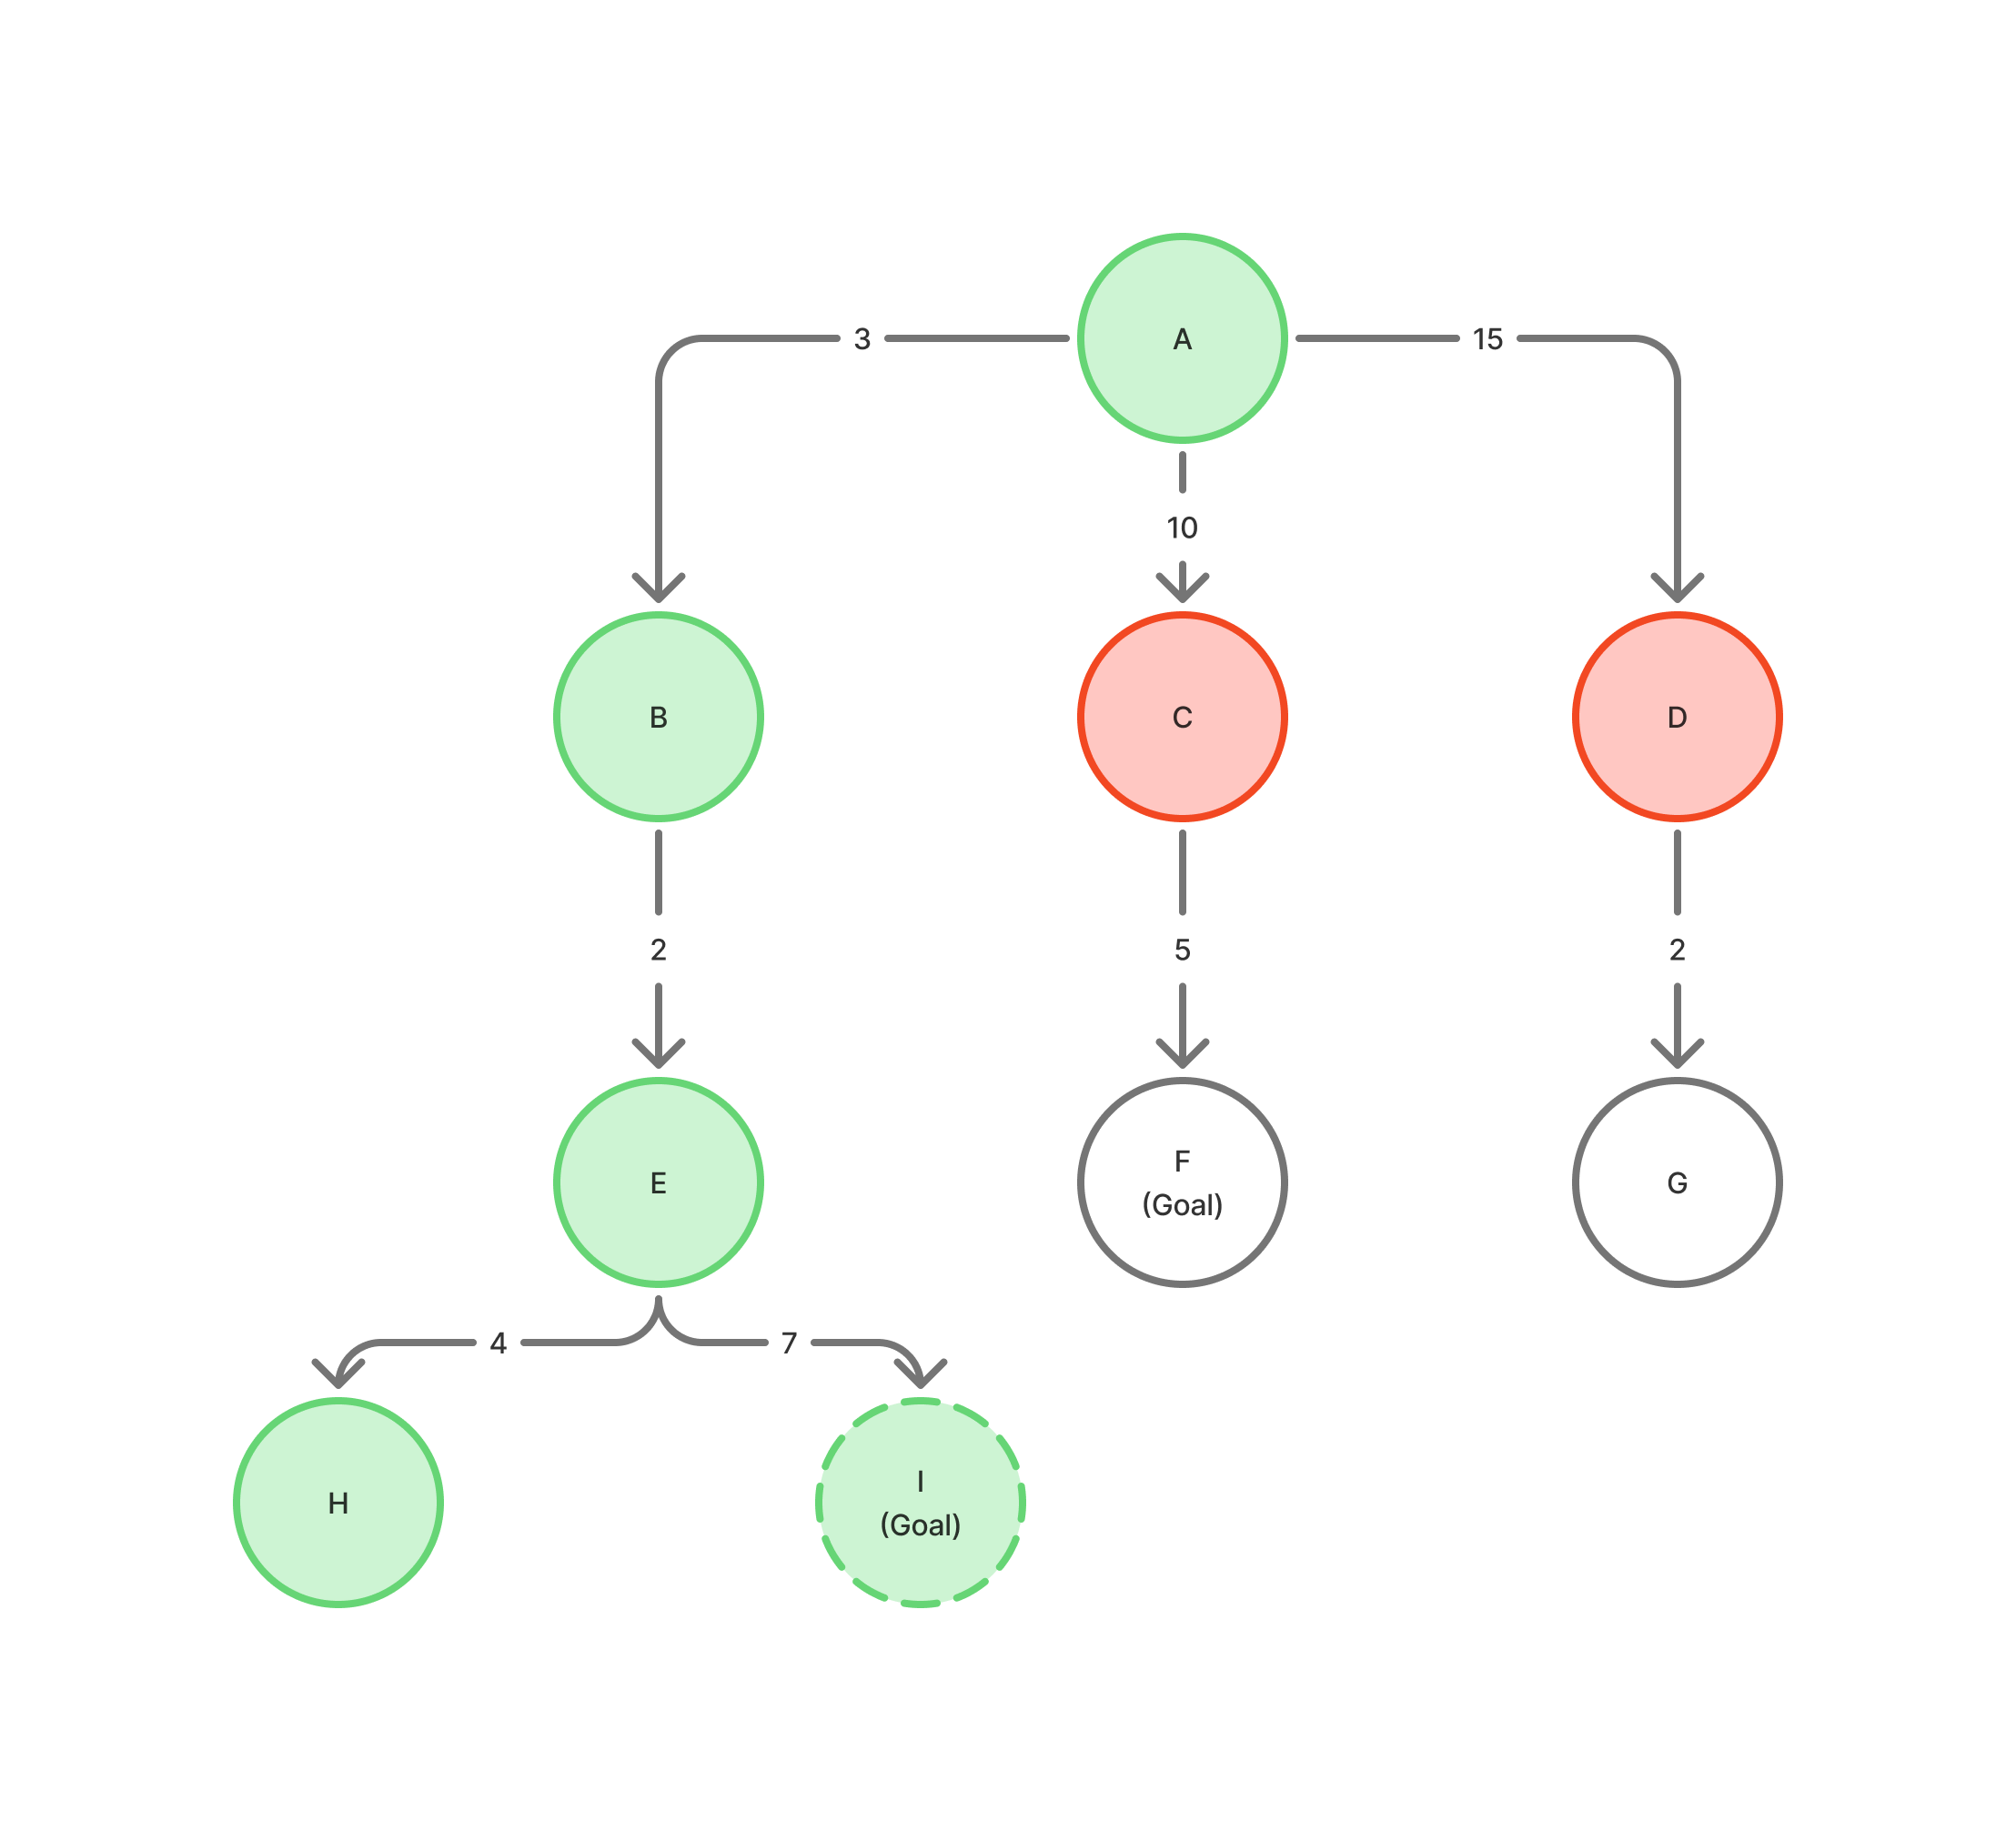
\includegraphics[width=2.08333in,height=\textheight,keepaspectratio]{./Dijakestria.gif}

}

\caption{Example of Uniform Search / Dijkstra's Algorithm}

\end{figure}%

\subsubsection{Bidirectional Search}\label{bidirectional-search}

Bidirectional search: A search technique where two searches are
initialized, one from the beginning and one from the end.

\begin{itemize}
\tightlist
\item
  It on average cuts the time by the \(\sqrt{x}\) where x is the cost of
  regular search
\end{itemize}

Bidirectional search should be used if the following conditions are met:

\begin{verbatim}
    1. Goal state is known ahead of time and unique.
    2. States are easily checked for equality (know when the two states meet up).
    3. Transition function must be easily invertible.
    4. (Optional) Are able to search concurrently (Two different cores) or you would need to context switch between the two searches.
\end{verbatim}

\begin{tcolorbox}[enhanced jigsaw, opacitybacktitle=0.6, title=\textcolor{quarto-callout-note-color}{\faInfo}\hspace{0.5em}{Note}, toptitle=1mm, left=2mm, breakable, titlerule=0mm, bottomtitle=1mm, bottomrule=.15mm, leftrule=.75mm, colframe=quarto-callout-note-color-frame, arc=.35mm, rightrule=.15mm, toprule=.15mm, coltitle=black, colback=white, opacityback=0, colbacktitle=quarto-callout-note-color!10!white]

You need to store the ``frontier'' to know if you have a convergence
point, therefore bidirectional search is done with BFS

\begin{verbatim}
 - You can cache the preferred path for better efficiency 
\end{verbatim}

\end{tcolorbox}

The following is a chart outlining different:

Uninformed Search, Their Advantages and Subsequent Costs

\begin{longtable}[]{@{}
  >{\centering\arraybackslash}p{(\linewidth - 12\tabcolsep) * \real{0.1429}}
  >{\centering\arraybackslash}p{(\linewidth - 12\tabcolsep) * \real{0.1429}}
  >{\centering\arraybackslash}p{(\linewidth - 12\tabcolsep) * \real{0.1429}}
  >{\centering\arraybackslash}p{(\linewidth - 12\tabcolsep) * \real{0.1429}}
  >{\centering\arraybackslash}p{(\linewidth - 12\tabcolsep) * \real{0.1429}}
  >{\centering\arraybackslash}p{(\linewidth - 12\tabcolsep) * \real{0.1429}}
  >{\centering\arraybackslash}p{(\linewidth - 12\tabcolsep) * \real{0.1429}}@{}}
\toprule\noalign{}
\begin{minipage}[b]{\linewidth}\centering
Method
\end{minipage} & \begin{minipage}[b]{\linewidth}\centering
Complete?
\end{minipage} & \begin{minipage}[b]{\linewidth}\centering
Optimal?
\end{minipage} & \begin{minipage}[b]{\linewidth}\centering
Space Complexity
\end{minipage} & \begin{minipage}[b]{\linewidth}\centering
Time complexity
\end{minipage} & \begin{minipage}[b]{\linewidth}\centering
Data structure for fringe
\end{minipage} & \begin{minipage}[b]{\linewidth}\centering
Notes
\end{minipage} \\
\midrule\noalign{}
\endhead
\bottomrule\noalign{}
\endlastfoot
BFS & Yes (finite b) & Yes (if costs are constant) & Exponential &
Exponential & FIFO (queue) & Complete, Optimal, bad memory complexity \\
Uniform-Cost & Yes & Yes (even it variable costs) exponential &
Exponential & Exponential & Priority Queue & Handles different costs \\
DFS & No & No & linear \textasciitilde{} b*m & Exponential & LIFO
(stack) & Low memory requirement, but fewer guarantees than BFS \\
Backtracking DFS & No & No & linear \textasciitilde{} m & Exponential &
Only 1 node in fringe (but may use stack as part of backtracking
implementation) & Even lower memory requirement, but a bit more
complicated than DFS \\
Depth-Limited & No & No & Linear \textasciitilde{} bl & Exponential &
Stack (variation of BFS) & Alleviates DFS problems with infinite spaces
and loops \\
Iterative Deepening & Yes (if reachable with available memory) & Yes (if
reachable with available memory) & Linear \textasciitilde{} bd &
Exponential & Stack (variation of BFS) & Combines low memory of DFS with
completeness and optimality of BFS. Re- explores shallow nodes many
times (not too bad) \\
Bi-directional & Yes (if using BFS) & Yes (if using BFS) & Exponential
(square root of complexity with BFS) & Exponential (square root of
complexity with most other strategies) & Depends on which strategy each
side is using & Needs to generate predecessors, needs to enumerate
goals, at least one side needs to store all frontier nodes \\
\end{longtable}

\subsection{Informed Search}\label{informed-search}

\begin{description}
\tightlist
\item[Informed Search]
Is the processes of adding a heuristic or estimate on how close we are
(cost of reaching ) a end state.
\end{description}

In general, informed search performs better than uniformed search.

\begin{tcolorbox}[enhanced jigsaw, opacitybacktitle=0.6, title=\textcolor{quarto-callout-note-color}{\faInfo}\hspace{0.5em}{Note}, toptitle=1mm, left=2mm, breakable, titlerule=0mm, bottomtitle=1mm, bottomrule=.15mm, leftrule=.75mm, colframe=quarto-callout-note-color-frame, arc=.35mm, rightrule=.15mm, toprule=.15mm, coltitle=black, colback=white, opacityback=0, colbacktitle=quarto-callout-note-color!10!white]

In the following section assume the heuristics is given

\end{tcolorbox}

\begin{tcolorbox}[enhanced jigsaw, opacitybacktitle=0.6, title=\textcolor{quarto-callout-warning-color}{\faExclamationTriangle}\hspace{0.5em}{Warning}, toptitle=1mm, left=2mm, breakable, titlerule=0mm, bottomtitle=1mm, bottomrule=.15mm, leftrule=.75mm, colframe=quarto-callout-warning-color-frame, arc=.35mm, rightrule=.15mm, toprule=.15mm, coltitle=black, colback=white, opacityback=0, colbacktitle=quarto-callout-warning-color!10!white]

Heuristics does not solve all problems for large datasets such as chess
heuristics still does not provide the capability to search the entire
possible game space.

\end{tcolorbox}

\texttt{F(n)}n is a function that \textbf{estimates}\footnote{How do you
  know what is best though? You \textbf{dent}, so you estimate by an
  heuristics} how useful a particular node is.

\begin{tcolorbox}[enhanced jigsaw, toprule=.15mm, left=2mm, breakable, arc=.35mm, rightrule=.15mm, bottomrule=.15mm, leftrule=.75mm, colframe=quarto-callout-color-frame, opacityback=0, colback=white]

\begin{itemize}
\item
  \begin{description}
  \tightlist
  \item[\texttt{N}]
  A node in the queue ready to be explored.
  \end{description}
\item
  \begin{description}
  \tightlist
  \item[\texttt{F(n)}]
  An estimate of how good it is to expand the node.
  \end{description}
\item
  \begin{description}
  \tightlist
  \item[\texttt{G(n)}]
  The true cost from the root to the current node.
  \end{description}
\item
  \begin{description}
  \tightlist
  \item[\texttt{H(n)}]
  An estimate of the cost of the best path from n -\textgreater{} goal
  node.
  \end{description}
\end{itemize}

\end{tcolorbox}

Uninformed search is a variation of informed search where \texttt{F(n)}
= \texttt{G(n)}

\subsubsection{Greedy Algorithm}\label{greedy-algorithm}

\begin{description}
\tightlist
\item[Greedy Algorithm]
An search algorithm that bases its decision purely on heuristics;
ignoring all cost that are incurred to get to that node (ie
\texttt{G(n)} = \texttt{F(n)} )
\end{description}

\begin{tcolorbox}[enhanced jigsaw, opacitybacktitle=0.6, title=\textcolor{quarto-callout-warning-color}{\faExclamationTriangle}\hspace{0.5em}{Warning}, toptitle=1mm, left=2mm, breakable, titlerule=0mm, bottomtitle=1mm, bottomrule=.15mm, leftrule=.75mm, colframe=quarto-callout-warning-color-frame, arc=.35mm, rightrule=.15mm, toprule=.15mm, coltitle=black, colback=white, opacityback=0, colbacktitle=quarto-callout-warning-color!10!white]

Greedy is incomplete just like DFS as it gets stuck on loops, or large
infinitely large graphs

\end{tcolorbox}

\begin{Shaded}
\begin{Highlighting}[]
\CommentTok{\# Fringe is sorted by node.heuristic in increasing order}
\CommentTok{\# ======== Note =============}
\CommentTok{\# The "win condition" heuristic is 0  }
\KeywordTok{def}\NormalTok{ greedy(root):}
\NormalTok{  fringe.enqueue(root)}
  \ControlFlowTok{while} \KeywordTok{not}\NormalTok{ fringe.empty():}
\NormalTok{    node }\OperatorTok{=}\NormalTok{ fringe.dequeue()}
    \ControlFlowTok{if}\NormalTok{(isWin(node)):}
      \ControlFlowTok{return}\NormalTok{ node}
    \ControlFlowTok{else}\NormalTok{:}
      \ControlFlowTok{for}\NormalTok{ child }\KeywordTok{in}\NormalTok{ node.children:}
\NormalTok{        fringe.enqueue(child)}
  \ControlFlowTok{return} \VariableTok{None}
\end{Highlighting}
\end{Shaded}

\paragraph{When Should You use
Greedy?}\label{when-should-you-use-greedy}

\begin{enumerate}
\def\labelenumi{\arabic{enumi}.}
\tightlist
\item
  Your heuristics are really good
\item
  Faster than \texttt{A\ *} if a solution can be found in a similar
  number of steps
\item
  Resource limited like in embedded systems less resource intensive as
  \texttt{A\ *}
\item
  If cost of search is more important than Optimality of a search
\item
  The cost to current node is sunken in or backtracking is
  costly/unnecessary
\end{enumerate}

\textbf{NOTE} Even though a solution is found its not optimal as greedy
stops as soon as a solution.

\subsubsection{A *}\label{a}

\begin{description}
\tightlist
\item[A Star (\texttt{*})]
A search algorithm that combines the advantages and techniques of both
greedy and Dijkstra algorithms. Its commonly used in industry for
patting, mapping and gaming applications. \texttt{F(n)} = \texttt{G(n)}
+ \texttt{H(n)}
\end{description}

\begin{tcolorbox}[enhanced jigsaw, toprule=.15mm, left=2mm, breakable, arc=.35mm, rightrule=.15mm, bottomrule=.15mm, leftrule=.75mm, colframe=quarto-callout-color-frame, opacityback=0, colback=white]

\begin{itemize}
\item
  \begin{description}
  \tightlist
  \item[\texttt{G(n)}]
  The true cost from the root to the current node.
  \end{description}
\item
  \begin{description}
  \tightlist
  \item[\texttt{H(n)}]
  An heuristic function that estimates how far away the current position
  is from the goal
  \end{description}
\end{itemize}

\end{tcolorbox}

\begin{Shaded}
\begin{Highlighting}[]
\CommentTok{\# Fringe is sorted by node.value in increasing order}
\CommentTok{\# ======== Note =============}
\CommentTok{\# Root\textquotesingle{}s cost is 0}
\CommentTok{\# The "win condition" heuristic is 0  }
\KeywordTok{def}\NormalTok{ aStar(root):}
\NormalTok{  fringe.enqueue(root)}
  \ControlFlowTok{while} \KeywordTok{not}\NormalTok{ fringe.empty():}
\NormalTok{    node }\OperatorTok{=}\NormalTok{ fringe.dequeue()}
    \ControlFlowTok{if}\NormalTok{(isWin(node)):}
      \ControlFlowTok{return}\NormalTok{ node}
    \ControlFlowTok{else}\NormalTok{:}
      \ControlFlowTok{for}\NormalTok{ child }\KeywordTok{in}\NormalTok{ node.children:}
\NormalTok{        child.value }\OperatorTok{=}\NormalTok{ node.cost }\OperatorTok{+}\NormalTok{ child.heuristic }
\NormalTok{        fringe.enqueue(child)}
  \ControlFlowTok{return} \VariableTok{None}
\end{Highlighting}
\end{Shaded}

When a node is enqueued to the fringe its \texttt{f(n)} is calculated
and placed as metadata of the node

Even though a win condition can be seen in the queue, unlike
\hyperref[greedy-algorithm]{greedy} \texttt{A\ *} does not pick it
immediately, if there are nodes with lower \texttt{F(n)} values

However, we can eliminate all items in the queue that are greater than
\texttt{F(n)} of that node since we know at maximum we know a solution
at maximum would be \texttt{F(n)} of that node.

\newpage{}

\paragraph{Choosing Heuristics}\label{choosing-heuristics}

\begin{tcolorbox}[enhanced jigsaw, opacitybacktitle=0.6, title=\textcolor{quarto-callout-caution-color}{\faFire}\hspace{0.5em}{Caution}, toptitle=1mm, left=2mm, breakable, titlerule=0mm, bottomtitle=1mm, bottomrule=.15mm, leftrule=.75mm, colframe=quarto-callout-caution-color-frame, arc=.35mm, rightrule=.15mm, toprule=.15mm, coltitle=black, colback=white, opacityback=0, colbacktitle=quarto-callout-caution-color!10!white]

When choosing heuristics you should not chose heuristics that are an
overestimate of the real cost as it creates delusions

\begin{figure}[H]

{\centering 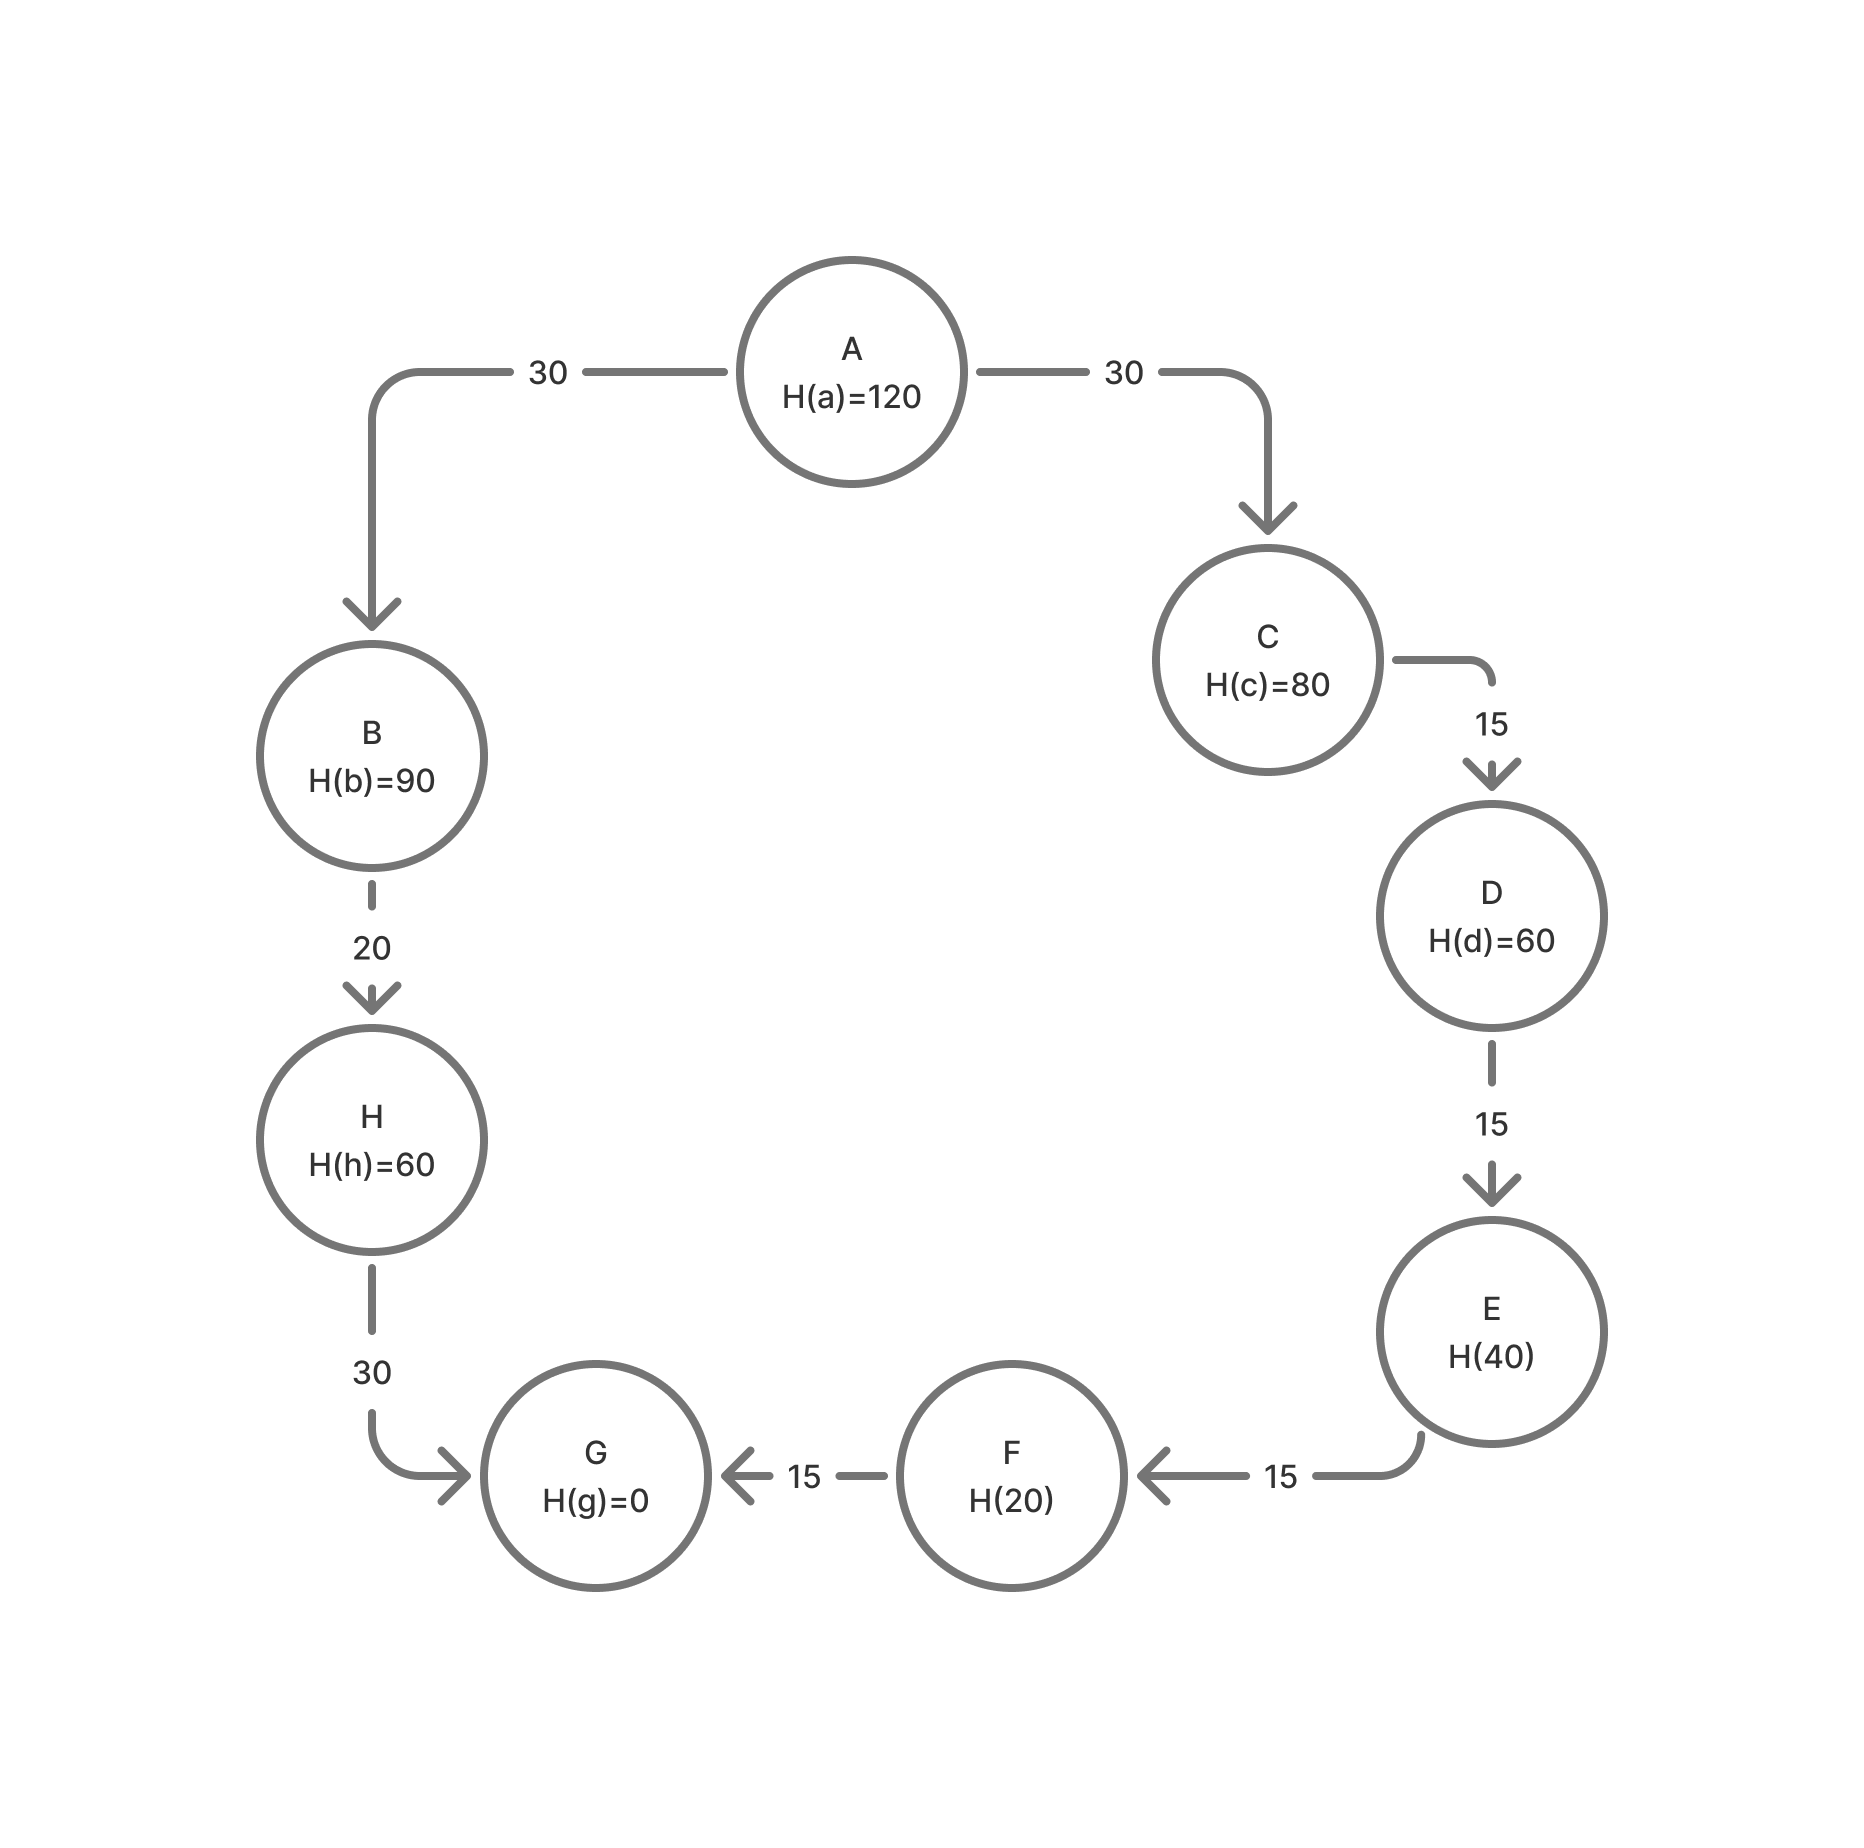
\includegraphics[width=2.08333in,height=\textheight,keepaspectratio]{./nop.png}

}

\caption{The following example shows an example of an \textbf{over
estimate} of heuristics which would make A * waste time discovering an
non-optimal route}

\end{figure}%

\end{tcolorbox}

\begin{tcolorbox}[enhanced jigsaw, opacitybacktitle=0.6, title=\textcolor{quarto-callout-tip-color}{\faLightbulb}\hspace{0.5em}{Tip}, toptitle=1mm, left=2mm, breakable, titlerule=0mm, bottomtitle=1mm, bottomrule=.15mm, leftrule=.75mm, colframe=quarto-callout-tip-color-frame, arc=.35mm, rightrule=.15mm, toprule=.15mm, coltitle=black, colback=white, opacityback=0, colbacktitle=quarto-callout-tip-color!10!white]

A common way to chose an heuristic is to pick the \textbf{optimal} best
case scenario (ie a world you have no challenges/obstacle/rules to
prevent you reaching your goal)

\end{tcolorbox}

\subparagraph{\texorpdfstring{Common Heuristics for
\texttt{A\ *}}{Common Heuristics for A *}}\label{common-heuristics-for-a}

\begin{itemize}
\item
  \begin{description}
  \tightlist
  \item[Euclidean Distance]
  The diagonal or crow distance between any two points on a 2/3D grid,
  calculated by the distance formula d =
  \(\sqrt{(x_2 - x_1)^2 + (y_2 - y_1)^2 + (z_2 - z_1)^2}\)
  \end{description}
\item
  \begin{description}
  \tightlist
  \item[ Manhattan Distance]
  The total distance between two points on a 2/3D where valid movement
  can only be in one axis at a time d =
  \(|(x_2 - x_1)| + |(y_2 - y_1)| + |(z_2 - z_1)|\)
  \end{description}
\end{itemize}

In general, manhattan distance is a better distance heuristic for (for
most situations) modeling realistic patting since its rare than you can
move in two (or more) directions at once.

\paragraph{Admissible Heuristics}\label{admissible-heuristics}

\begin{itemize}
\tightlist
\item
  Admissible Heuristics: A heuristics is admissible if it underestimates
  or equals the true cost from the current node to the end node.
\end{itemize}

\begin{tcolorbox}[enhanced jigsaw, opacitybacktitle=0.6, title=\textcolor{quarto-callout-tip-color}{\faLightbulb}\hspace{0.5em}{Tip}, toptitle=1mm, left=2mm, breakable, titlerule=0mm, bottomtitle=1mm, bottomrule=.15mm, leftrule=.75mm, colframe=quarto-callout-tip-color-frame, arc=.35mm, rightrule=.15mm, toprule=.15mm, coltitle=black, colback=white, opacityback=0, colbacktitle=quarto-callout-tip-color!10!white]

If you have multiple admissible heuristics from A --\textgreater{} B
then the \textbf{maximum} of those heuristics as it most closely mimics
the real cost from A --\textgreater{} B

\end{tcolorbox}

\subparagraph{Example with 8 Puzzle}\label{example-with-8-puzzle}

8 Puzzle is a sliding board puzzle where there are 8 numbered pieces on
a \texttt{3\ x\ 3} board. The goal is to arrange the puzzle pieces in a
specific order such as

\begin{longtable}[]{@{}
  >{\centering\arraybackslash}p{(\linewidth - 2\tabcolsep) * \real{0.5000}}
  >{\centering\arraybackslash}p{(\linewidth - 2\tabcolsep) * \real{0.5000}}@{}}
\toprule\noalign{}
\begin{minipage}[b]{\linewidth}\centering
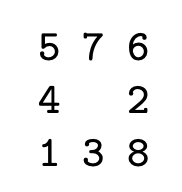
\includegraphics[width=1.04167in,height=\textheight,keepaspectratio]{./unsolved.png}
\end{minipage} & \begin{minipage}[b]{\linewidth}\centering
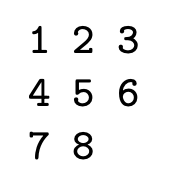
\includegraphics[width=1.04167in,height=\textheight,keepaspectratio]{./solved.png}
\end{minipage} \\
\midrule\noalign{}
\endhead
\bottomrule\noalign{}
\endlastfoot
\emph{Original 8 Puzzle Ex} & \emph{Solved 8 Puzzle Ex} \\
\end{longtable}

Two common heuristics used in 8 puzzle:

\begin{enumerate}
\def\labelenumi{\arabic{enumi}.}
\tightlist
\item
  Number of misplaced pieces
\item
  The manhattan distance between the current position and the correct
  position
\end{enumerate}

In this scenario the \hyperref[manhattan_distance]{manhattan distance}
would be a more realistic and therefore dominant heuristic as in the
game only a piece can only be moved to an adjacent cell thats open. The
manhattan distance would represents the number of attempts in the
\textbf{ideal} configuration played perfectly.




\end{document}
